\documentclass[]{article}
\usepackage{lmodern}
\usepackage{amssymb,amsmath}
\usepackage{ifxetex,ifluatex}
\usepackage{fixltx2e} % provides \textsubscript
\ifnum 0\ifxetex 1\fi\ifluatex 1\fi=0 % if pdftex
  \usepackage[T1]{fontenc}
  \usepackage[utf8]{inputenc}
\else % if luatex or xelatex
  \ifxetex
    \usepackage{mathspec}
  \else
    \usepackage{fontspec}
  \fi
  \defaultfontfeatures{Ligatures=TeX,Scale=MatchLowercase}
\fi
% use upquote if available, for straight quotes in verbatim environments
\IfFileExists{upquote.sty}{\usepackage{upquote}}{}
% use microtype if available
\IfFileExists{microtype.sty}{%
\usepackage{microtype}
\UseMicrotypeSet[protrusion]{basicmath} % disable protrusion for tt fonts
}{}
\usepackage[margin=1in]{geometry}
\usepackage{hyperref}
\hypersetup{unicode=true,
            pdftitle={Lab3},
            pdfauthor={Kevin Luo},
            pdfborder={0 0 0},
            breaklinks=true}
\urlstyle{same}  % don't use monospace font for urls
\usepackage{color}
\usepackage{fancyvrb}
\newcommand{\VerbBar}{|}
\newcommand{\VERB}{\Verb[commandchars=\\\{\}]}
\DefineVerbatimEnvironment{Highlighting}{Verbatim}{commandchars=\\\{\}}
% Add ',fontsize=\small' for more characters per line
\usepackage{framed}
\definecolor{shadecolor}{RGB}{248,248,248}
\newenvironment{Shaded}{\begin{snugshade}}{\end{snugshade}}
\newcommand{\KeywordTok}[1]{\textcolor[rgb]{0.13,0.29,0.53}{\textbf{#1}}}
\newcommand{\DataTypeTok}[1]{\textcolor[rgb]{0.13,0.29,0.53}{#1}}
\newcommand{\DecValTok}[1]{\textcolor[rgb]{0.00,0.00,0.81}{#1}}
\newcommand{\BaseNTok}[1]{\textcolor[rgb]{0.00,0.00,0.81}{#1}}
\newcommand{\FloatTok}[1]{\textcolor[rgb]{0.00,0.00,0.81}{#1}}
\newcommand{\ConstantTok}[1]{\textcolor[rgb]{0.00,0.00,0.00}{#1}}
\newcommand{\CharTok}[1]{\textcolor[rgb]{0.31,0.60,0.02}{#1}}
\newcommand{\SpecialCharTok}[1]{\textcolor[rgb]{0.00,0.00,0.00}{#1}}
\newcommand{\StringTok}[1]{\textcolor[rgb]{0.31,0.60,0.02}{#1}}
\newcommand{\VerbatimStringTok}[1]{\textcolor[rgb]{0.31,0.60,0.02}{#1}}
\newcommand{\SpecialStringTok}[1]{\textcolor[rgb]{0.31,0.60,0.02}{#1}}
\newcommand{\ImportTok}[1]{#1}
\newcommand{\CommentTok}[1]{\textcolor[rgb]{0.56,0.35,0.01}{\textit{#1}}}
\newcommand{\DocumentationTok}[1]{\textcolor[rgb]{0.56,0.35,0.01}{\textbf{\textit{#1}}}}
\newcommand{\AnnotationTok}[1]{\textcolor[rgb]{0.56,0.35,0.01}{\textbf{\textit{#1}}}}
\newcommand{\CommentVarTok}[1]{\textcolor[rgb]{0.56,0.35,0.01}{\textbf{\textit{#1}}}}
\newcommand{\OtherTok}[1]{\textcolor[rgb]{0.56,0.35,0.01}{#1}}
\newcommand{\FunctionTok}[1]{\textcolor[rgb]{0.00,0.00,0.00}{#1}}
\newcommand{\VariableTok}[1]{\textcolor[rgb]{0.00,0.00,0.00}{#1}}
\newcommand{\ControlFlowTok}[1]{\textcolor[rgb]{0.13,0.29,0.53}{\textbf{#1}}}
\newcommand{\OperatorTok}[1]{\textcolor[rgb]{0.81,0.36,0.00}{\textbf{#1}}}
\newcommand{\BuiltInTok}[1]{#1}
\newcommand{\ExtensionTok}[1]{#1}
\newcommand{\PreprocessorTok}[1]{\textcolor[rgb]{0.56,0.35,0.01}{\textit{#1}}}
\newcommand{\AttributeTok}[1]{\textcolor[rgb]{0.77,0.63,0.00}{#1}}
\newcommand{\RegionMarkerTok}[1]{#1}
\newcommand{\InformationTok}[1]{\textcolor[rgb]{0.56,0.35,0.01}{\textbf{\textit{#1}}}}
\newcommand{\WarningTok}[1]{\textcolor[rgb]{0.56,0.35,0.01}{\textbf{\textit{#1}}}}
\newcommand{\AlertTok}[1]{\textcolor[rgb]{0.94,0.16,0.16}{#1}}
\newcommand{\ErrorTok}[1]{\textcolor[rgb]{0.64,0.00,0.00}{\textbf{#1}}}
\newcommand{\NormalTok}[1]{#1}
\usepackage{graphicx,grffile}
\makeatletter
\def\maxwidth{\ifdim\Gin@nat@width>\linewidth\linewidth\else\Gin@nat@width\fi}
\def\maxheight{\ifdim\Gin@nat@height>\textheight\textheight\else\Gin@nat@height\fi}
\makeatother
% Scale images if necessary, so that they will not overflow the page
% margins by default, and it is still possible to overwrite the defaults
% using explicit options in \includegraphics[width, height, ...]{}
\setkeys{Gin}{width=\maxwidth,height=\maxheight,keepaspectratio}
\IfFileExists{parskip.sty}{%
\usepackage{parskip}
}{% else
\setlength{\parindent}{0pt}
\setlength{\parskip}{6pt plus 2pt minus 1pt}
}
\setlength{\emergencystretch}{3em}  % prevent overfull lines
\providecommand{\tightlist}{%
  \setlength{\itemsep}{0pt}\setlength{\parskip}{0pt}}
\setcounter{secnumdepth}{0}
% Redefines (sub)paragraphs to behave more like sections
\ifx\paragraph\undefined\else
\let\oldparagraph\paragraph
\renewcommand{\paragraph}[1]{\oldparagraph{#1}\mbox{}}
\fi
\ifx\subparagraph\undefined\else
\let\oldsubparagraph\subparagraph
\renewcommand{\subparagraph}[1]{\oldsubparagraph{#1}\mbox{}}
\fi

%%% Use protect on footnotes to avoid problems with footnotes in titles
\let\rmarkdownfootnote\footnote%
\def\footnote{\protect\rmarkdownfootnote}

%%% Change title format to be more compact
\usepackage{titling}

% Create subtitle command for use in maketitle
\providecommand{\subtitle}[1]{
  \posttitle{
    \begin{center}\large#1\end{center}
    }
}

\setlength{\droptitle}{-2em}

  \title{Lab3}
    \pretitle{\vspace{\droptitle}\centering\huge}
  \posttitle{\par}
    \author{Kevin Luo}
    \preauthor{\centering\large\emph}
  \postauthor{\par}
      \predate{\centering\large\emph}
  \postdate{\par}
    \date{2019/9/23}


\begin{document}
\maketitle

\section*{Part 1: Minimizing a quadratic}\subsubsection*{1.1}

\begin{Shaded}
\begin{Highlighting}[]
\NormalTok{f <-}\StringTok{ }\ControlFlowTok{function}\NormalTok{(x)\{}
  \KeywordTok{return}\NormalTok{(}\FloatTok{0.5}\OperatorTok{*}\NormalTok{(x}\OperatorTok{-}\DecValTok{2}\NormalTok{)}\OperatorTok{^}\DecValTok{2}\OperatorTok{+}\DecValTok{1}\NormalTok{)}
\NormalTok{\}}
\NormalTok{df <-}\StringTok{ }\ControlFlowTok{function}\NormalTok{(x)\{}
  \KeywordTok{return}\NormalTok{(x}\OperatorTok{-}\DecValTok{2}\NormalTok{)}
\NormalTok{\}}
\NormalTok{temp <-}\StringTok{ }\KeywordTok{seq}\NormalTok{(}\DecValTok{0}\NormalTok{,}\DecValTok{4}\NormalTok{,}\FloatTok{0.01}\NormalTok{)}
\NormalTok{tempplotf <-}\StringTok{ }\KeywordTok{data.frame}\NormalTok{(}\DataTypeTok{x =}\NormalTok{ temp, }\DataTypeTok{y =} \KeywordTok{f}\NormalTok{(temp))}
\NormalTok{tempplotdf <-}\StringTok{ }\KeywordTok{data.frame}\NormalTok{(}\DataTypeTok{x =}\NormalTok{ temp, }\DataTypeTok{y =} \KeywordTok{df}\NormalTok{(temp))}
\NormalTok{tempplotf }\OperatorTok\StringTok{ }\KeywordTok{ggplot}\NormalTok{() }\OperatorTok{+}\StringTok{ }\KeywordTok{theme_bw}\NormalTok{() }\OperatorTok{+}
\StringTok{  }\KeywordTok{geom_point}\NormalTok{(}\KeywordTok{aes}\NormalTok{(}\DataTypeTok{x =}\NormalTok{ x, }\DataTypeTok{y =}\NormalTok{ y), }\DataTypeTok{color =} \StringTok{'maroon'}\NormalTok{)}
\end{Highlighting}
\end{Shaded}

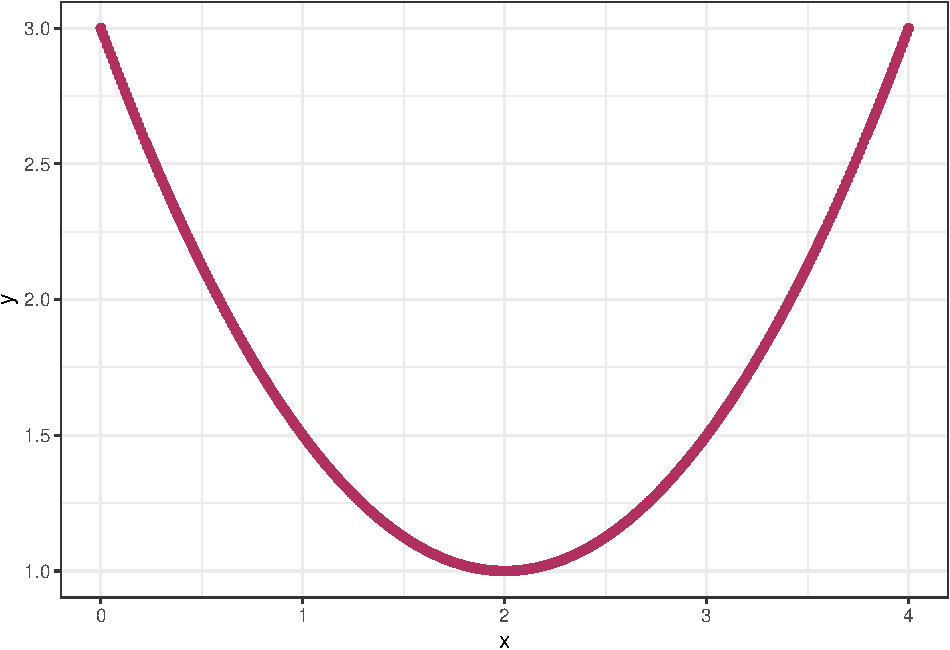
\includegraphics{lab3_files/figure-latex/unnamed-chunk-1-1.pdf}

\begin{Shaded}
\begin{Highlighting}[]
\NormalTok{tempplotdf }\OperatorTok\StringTok{ }\KeywordTok{ggplot}\NormalTok{() }\OperatorTok{+}\StringTok{ }\KeywordTok{theme_bw}\NormalTok{() }\OperatorTok{+}
\StringTok{  }\KeywordTok{geom_point}\NormalTok{(}\KeywordTok{aes}\NormalTok{(}\DataTypeTok{x =}\NormalTok{ x, }\DataTypeTok{y =}\NormalTok{ y), }\DataTypeTok{color =} \StringTok{'maroon'}\NormalTok{)}
\end{Highlighting}
\end{Shaded}

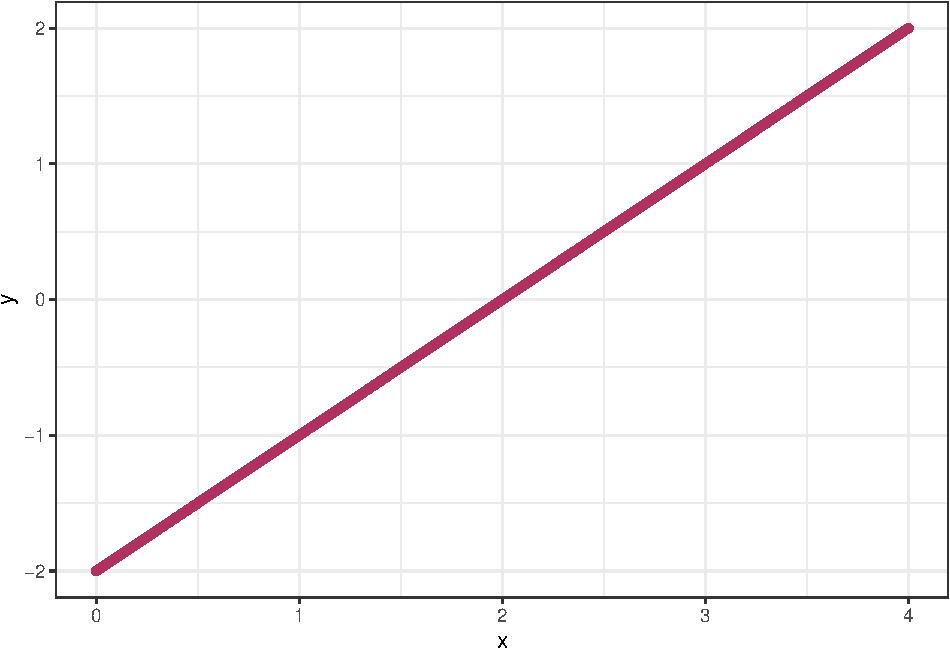
\includegraphics{lab3_files/figure-latex/unnamed-chunk-1-2.pdf}

\subsubsection*{1.2}

\begin{Shaded}
\begin{Highlighting}[]
\NormalTok{x =}\StringTok{ }\KeywordTok{rnorm}\NormalTok{(}\DecValTok{1}\NormalTok{)}
\NormalTok{alpha =}\StringTok{ }\DecValTok{1}
\ControlFlowTok{for}\NormalTok{ (i }\ControlFlowTok{in} \DecValTok{1}\OperatorTok{:}\DecValTok{10}\NormalTok{)\{}
\NormalTok{  x =}\StringTok{ }\NormalTok{x }\OperatorTok{-}\StringTok{ }\NormalTok{alpha}\OperatorTok{*}\KeywordTok{df}\NormalTok{(x)}
\NormalTok{\}}
\NormalTok{x}
\end{Highlighting}
\end{Shaded}

\begin{verbatim}
## [1] 2
\end{verbatim}

\begin{Shaded}
\begin{Highlighting}[]
\CommentTok{# x = 2 is obviously the minimum for f(x)}
\end{Highlighting}
\end{Shaded}

\subsubsection*{1.3}

\begin{Shaded}
\begin{Highlighting}[]
\NormalTok{alpha <-}\StringTok{ }\FloatTok{0.1}
\NormalTok{x <-}\StringTok{ }\KeywordTok{rnorm}\NormalTok{(}\DecValTok{2}\NormalTok{)}
\NormalTok{A <-}\StringTok{ }\KeywordTok{diag}\NormalTok{(}\KeywordTok{c}\NormalTok{(}\DecValTok{1}\NormalTok{,}\DecValTok{2}\NormalTok{), }\DataTypeTok{nrow =} \DecValTok{2}\NormalTok{)}
\NormalTok{b <-}\StringTok{ }\KeywordTok{matrix}\NormalTok{(}\KeywordTok{c}\NormalTok{(}\DecValTok{1}\NormalTok{,}\DecValTok{1}\NormalTok{), }\DataTypeTok{ncol =} \DecValTok{1}\NormalTok{)}
\ControlFlowTok{for}\NormalTok{ (i }\ControlFlowTok{in} \DecValTok{1}\OperatorTok{:}\DecValTok{100}\NormalTok{)\{}
\NormalTok{  x =}\StringTok{ }\NormalTok{x }\OperatorTok{-}\StringTok{ }\NormalTok{alpha}\OperatorTok{*}\NormalTok{(A }\OperatorTok\StringTok{ }\NormalTok{x }\OperatorTok{-}\StringTok{ }\NormalTok{b)}
\NormalTok{\}}
\NormalTok{x}
\end{Highlighting}
\end{Shaded}

\begin{verbatim}
##          [,1]
## [1,] 0.999963
## [2,] 0.500000
\end{verbatim}

\section*{Part 2: OLS Regression}

\begin{Shaded}
\begin{Highlighting}[]
\NormalTok{response <-}\StringTok{ 'mpg'}
\NormalTok{predictors <-}\StringTok{ }\KeywordTok{c}\NormalTok{(}\StringTok{'hp'}\NormalTok{, }\StringTok{'qsec'}\NormalTok{, }\StringTok{'wt'}\NormalTok{) }
\NormalTok{M <-}\StringTok{ }\KeywordTok{as.matrix}\NormalTok{(mtcars[ ,predictors]) }
\NormalTok{X <-}\StringTok{ }\KeywordTok{cbind}\NormalTok{(}\DataTypeTok{intercept =} \DecValTok{1}\NormalTok{, M)}
\NormalTok{y <-}\StringTok{ }\NormalTok{mtcars[ ,response]}
\NormalTok{y <-}\StringTok{ }\KeywordTok{as.matrix}\NormalTok{(y, }\DataTypeTok{ncol =} \DecValTok{1}\NormalTok{)}
\end{Highlighting}
\end{Shaded}

\begin{Shaded}
\begin{Highlighting}[]
\NormalTok{test <-}\StringTok{ }\KeywordTok{lm}\NormalTok{(mpg}\OperatorTok{~}\NormalTok{hp}\OperatorTok{+}\NormalTok{qsec}\OperatorTok{+}\NormalTok{wt, }\DataTypeTok{data =}\NormalTok{ mtcars)}
\NormalTok{test}\OperatorTok{$}\NormalTok{coefficients }\OperatorTok{/}\StringTok{ }\KeywordTok{length}\NormalTok{(y)}
\end{Highlighting}
\end{Shaded}

\begin{verbatim}
##  (Intercept)           hp         qsec           wt 
##  0.862828964 -0.000556946  0.015963553 -0.136212413
\end{verbatim}

\begin{Shaded}
\begin{Highlighting}[]
\NormalTok{MSE <-}\StringTok{ }\ControlFlowTok{function}\NormalTok{(beta)\{}
  \KeywordTok{return}\NormalTok{(}\KeywordTok{t}\NormalTok{(X }\OperatorTok\StringTok{ }\NormalTok{beta }\OperatorTok{-}\StringTok{ }\NormalTok{y) }\OperatorTok\StringTok{ }\NormalTok{(X }\OperatorTok\StringTok{ }\NormalTok{beta }\OperatorTok{-}\StringTok{ }\NormalTok{y) }\OperatorTok{/}\StringTok{ }\KeywordTok{nrow}\NormalTok{(X))}
\NormalTok{\}}
\NormalTok{dMSE <-}\StringTok{ }\ControlFlowTok{function}\NormalTok{(beta)\{}
  \KeywordTok{return}\NormalTok{(}\DecValTok{2} \OperatorTok{*}\StringTok{ }\NormalTok{(}\KeywordTok{t}\NormalTok{(X) }\OperatorTok\StringTok{ }\NormalTok{X }\OperatorTok\StringTok{ }\NormalTok{beta }\OperatorTok{-}\StringTok{ }\KeywordTok{t}\NormalTok{(X) }\OperatorTok\StringTok{ }\NormalTok{y) }\OperatorTok{/}\StringTok{ }\KeywordTok{nrow}\NormalTok{(X))}
\NormalTok{\}}
\end{Highlighting}
\end{Shaded}

\begin{Shaded}
\begin{Highlighting}[]
\NormalTok{beta <-}\StringTok{ }\KeywordTok{matrix}\NormalTok{(}\KeywordTok{rnorm}\NormalTok{(}\DecValTok{4}\NormalTok{), }\DataTypeTok{ncol =} \DecValTok{1}\NormalTok{)}
\NormalTok{alpha <-}\StringTok{ }\FloatTok{0.00001}
\NormalTok{iteration <-}\StringTok{ }\DecValTok{500}
\NormalTok{plotdata <-}\StringTok{ }\KeywordTok{data.frame}\NormalTok{(}\DataTypeTok{index =} \DecValTok{1}\OperatorTok{:}\NormalTok{iteration, }\DataTypeTok{MSE =} \KeywordTok{rep}\NormalTok{(}\DecValTok{0}\NormalTok{,iteration))}
\ControlFlowTok{for}\NormalTok{ (i }\ControlFlowTok{in} \DecValTok{1}\OperatorTok{:}\NormalTok{iteration)\{}
\NormalTok{  beta =}\StringTok{ }\NormalTok{beta }\OperatorTok{-}\StringTok{ }\NormalTok{alpha }\OperatorTok{*}\StringTok{ }\NormalTok{(}\KeywordTok{dMSE}\NormalTok{(beta))}
\NormalTok{  plotdata[i,}\StringTok{'MSE'}\NormalTok{] =}\StringTok{ }\KeywordTok{MSE}\NormalTok{(beta)}
\NormalTok{\}}
\NormalTok{plotdata }\OperatorTok
\StringTok{  }\KeywordTok{ggplot}\NormalTok{(}\KeywordTok{aes}\NormalTok{(}\DataTypeTok{x =}\NormalTok{ index, }\DataTypeTok{y =}\NormalTok{ MSE)) }\OperatorTok{+}\StringTok{ }\KeywordTok{theme_bw}\NormalTok{() }\OperatorTok{+}
\StringTok{  }\KeywordTok{geom_point}\NormalTok{(}\DataTypeTok{color =} \StringTok{'maroon'}\NormalTok{)}
\end{Highlighting}
\end{Shaded}

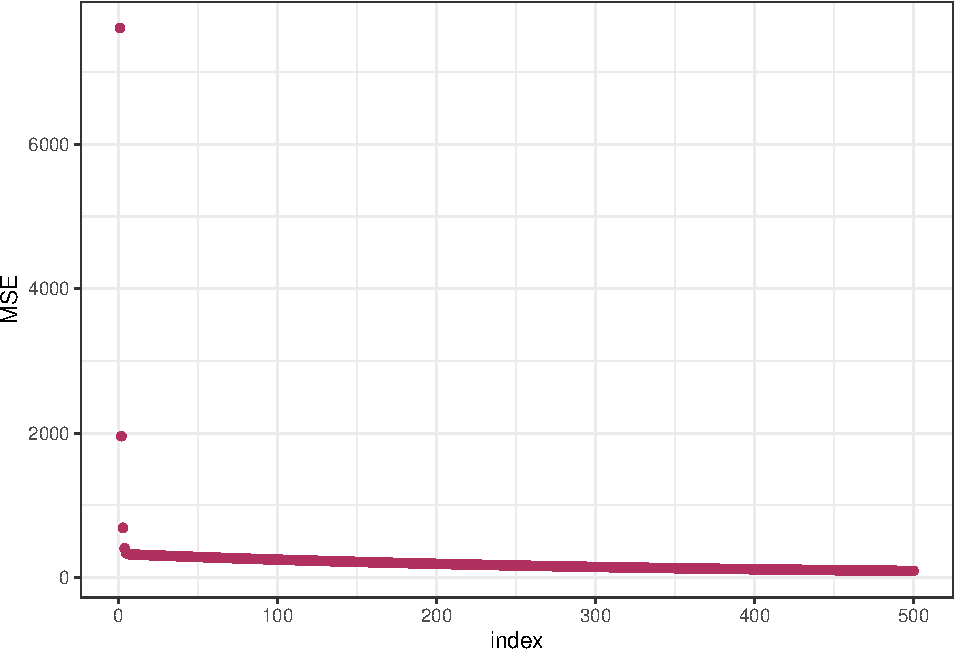
\includegraphics{lab3_files/figure-latex/unnamed-chunk-6-1.pdf}

\begin{Shaded}
\begin{Highlighting}[]
\NormalTok{sample_batch <-}\StringTok{ }\ControlFlowTok{function}\NormalTok{(n, B)\{}
  \KeywordTok{return}\NormalTok{(}\KeywordTok{sample}\NormalTok{(}\DecValTok{1}\OperatorTok{:}\NormalTok{n,B))}
\NormalTok{\}}
\NormalTok{B <-}\StringTok{ }\DecValTok{16}
\NormalTok{alpha <-}\StringTok{ }\FloatTok{0.00001}
\NormalTok{beta <-}\StringTok{ }\KeywordTok{matrix}\NormalTok{(}\KeywordTok{rnorm}\NormalTok{(}\DecValTok{4}\NormalTok{), }\DataTypeTok{ncol =} \DecValTok{1}\NormalTok{)}
\NormalTok{plotdata2 <-}\StringTok{ }\KeywordTok{data.frame}\NormalTok{(}\DataTypeTok{index =} \DecValTok{1}\OperatorTok{:}\NormalTok{iteration, }\DataTypeTok{MSE =} \KeywordTok{rep}\NormalTok{(}\DecValTok{0}\NormalTok{,iteration))}

\ControlFlowTok{for}\NormalTok{ (i }\ControlFlowTok{in} \DecValTok{1}\OperatorTok{:}\DecValTok{500}\NormalTok{)\{}
\NormalTok{  sampleRows <-}\StringTok{ }\KeywordTok{sample_batch}\NormalTok{(}\KeywordTok{nrow}\NormalTok{(X), B)}
\NormalTok{  tempX <-}\StringTok{ }\NormalTok{X[sampleRows,]}
\NormalTok{  tempy <-}\StringTok{ }\KeywordTok{matrix}\NormalTok{(y[sampleRows,], }\DataTypeTok{ncol =} \DecValTok{1}\NormalTok{)}
\NormalTok{  beta =}\StringTok{ }\NormalTok{beta }\OperatorTok{-}\StringTok{ }\NormalTok{alpha }\OperatorTok{*}\StringTok{ }\DecValTok{2} \OperatorTok{*}\StringTok{ }\NormalTok{(}\KeywordTok{t}\NormalTok{(tempX) }\OperatorTok\StringTok{ }\NormalTok{tempX }\OperatorTok\StringTok{ }\NormalTok{beta }\OperatorTok{-}\StringTok{ }\KeywordTok{t}\NormalTok{(tempX) }\OperatorTok\StringTok{ }\NormalTok{tempy) }\OperatorTok{/}\StringTok{ }\KeywordTok{nrow}\NormalTok{(tempy)}
\NormalTok{  plotdata2[i,}\StringTok{'MSE'}\NormalTok{] =}\StringTok{ }\KeywordTok{MSE}\NormalTok{(beta)}
\NormalTok{\}}
\NormalTok{beta}
\end{Highlighting}
\end{Shaded}

\begin{verbatim}
##                  [,1]
## intercept -0.07583735
## hp         0.02642154
## qsec       0.58433473
## wt         0.66847470
\end{verbatim}

\begin{Shaded}
\begin{Highlighting}[]
\NormalTok{plotdata2 }\OperatorTok
\StringTok{  }\KeywordTok{ggplot}\NormalTok{(}\KeywordTok{aes}\NormalTok{(}\DataTypeTok{x =}\NormalTok{ index, }\DataTypeTok{y =}\NormalTok{ MSE)) }\OperatorTok{+}\StringTok{ }\KeywordTok{theme_bw}\NormalTok{() }\OperatorTok{+}
\StringTok{  }\KeywordTok{geom_point}\NormalTok{(}\DataTypeTok{color =} \StringTok{'maroon'}\NormalTok{)}
\end{Highlighting}
\end{Shaded}

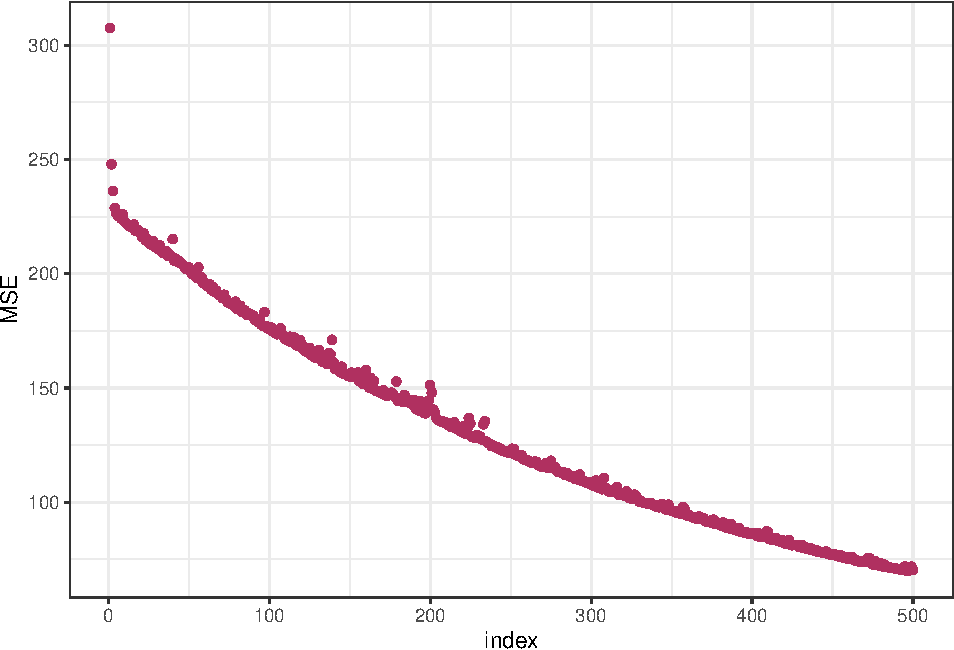
\includegraphics{lab3_files/figure-latex/unnamed-chunk-7-1.pdf}


\end{document}
